\section{Additional Training Table Statistics}\label{app: train table stats}

We report additional training table statistics for all tasks, separated into entity classification (\emph{cf.}~Table~\ref{tab:node_classification_stats}), entity regression (\emph{cf.}~Table~\ref{tab:node_regression_stats}), and link prediction (\emph{cf.}~Table~\ref{tab:link_prediction_stats}).

\begin{table}[H]
    \caption{\relbench entity classification training table target statistics.}
    \centering
    \setlength{\tabcolsep}{3pt}
    \scriptsize
    \CatchFileDef{\tabledata}{tables/node_classification_stats.tex}{}
    \begin{tabular}{llrrr}
    \toprule
    \textbf{Dataset} & \textbf{Task} & \textbf{Split} & \textbf{Positives} & \textbf{Negatives} \\
    \midrule
    \tabledata
    \bottomrule
    \end{tabular}
    \label{tab:node_classification_stats}
\end{table}

\begin{table}[H] 
    \caption{\relbench entity regression training table target statistics.}
    \centering
    \setlength{\tabcolsep}{3pt}
    \scriptsize
    \CatchFileDef{\tabledata}{tables/node_regression_stats.tex}{}
    \begin{tabular}{llrrrrr}
    \toprule
    \textbf{Dataset} & \textbf{Task} & \textbf{Split} & \textbf{Minimum} & \textbf{Median} & \textbf{Mean} & \textbf{Maximum} \\
    \midrule
    \tabledata
    \bottomrule
    \end{tabular}
    \label{tab:node_regression_stats}
\end{table}

\begin{table}[H]
    \caption{\relbench link prediction training table link statistics.}
    \centering
    \setlength{\tabcolsep}{3pt}
    \scriptsize
    \CatchFileDef{\tabledata}{tables/link_prediction_stats.tex}{}
    \begin{tabular}{llrrrr}
    \toprule
    \textbf{Dataset} & \textbf{Task} & \textbf{Split} & \textbf{\#Links} & \makecell{\textbf{Avg \#links per}\\\textbf{entity/timestamp}} & \textbf{\%Repeated links} \\
    \midrule
    \tabledata
    \bottomrule
    \end{tabular}
    \label{tab:link_prediction_stats}
\end{table}

\section{Dataset Schema}

\begin{figure}[H]
    \centering
    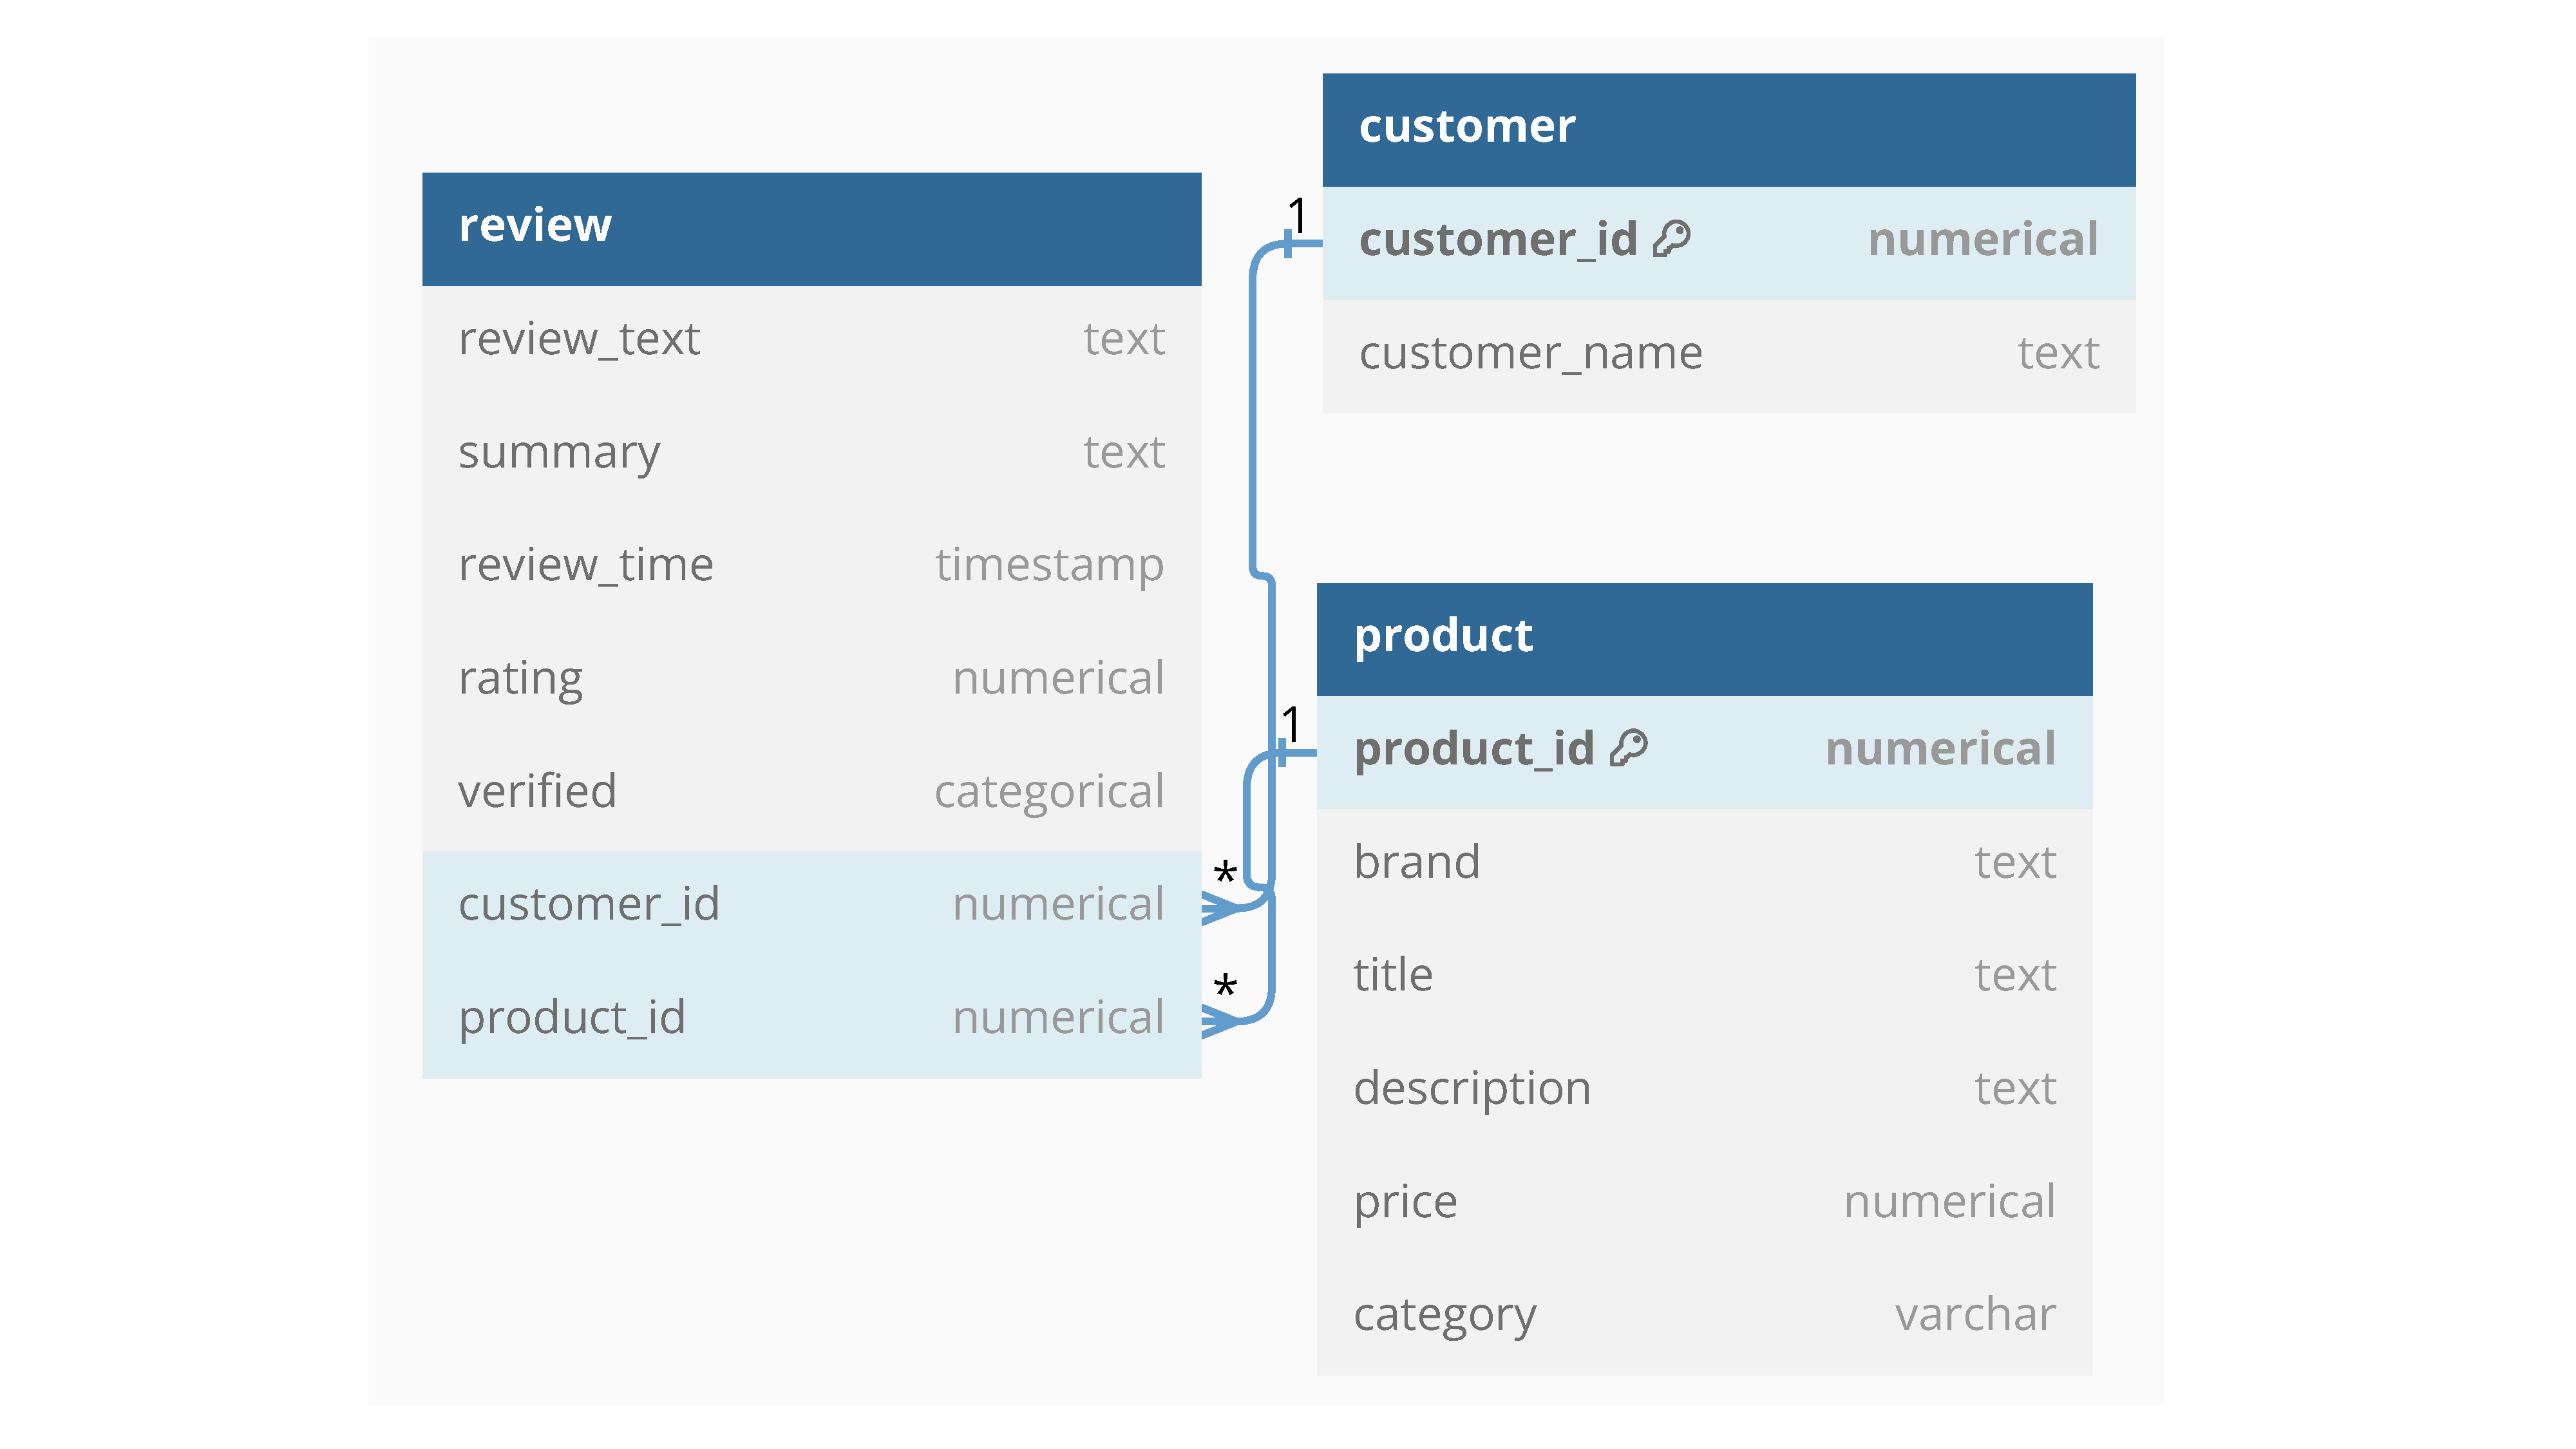
\includegraphics[width=0.6\textwidth]{figs/rel-amazon.pdf}
    \caption{\amazon database diagram.}
    \label{fig:amazon-db}
\end{figure}

\begin{figure}[H]
    \centering
    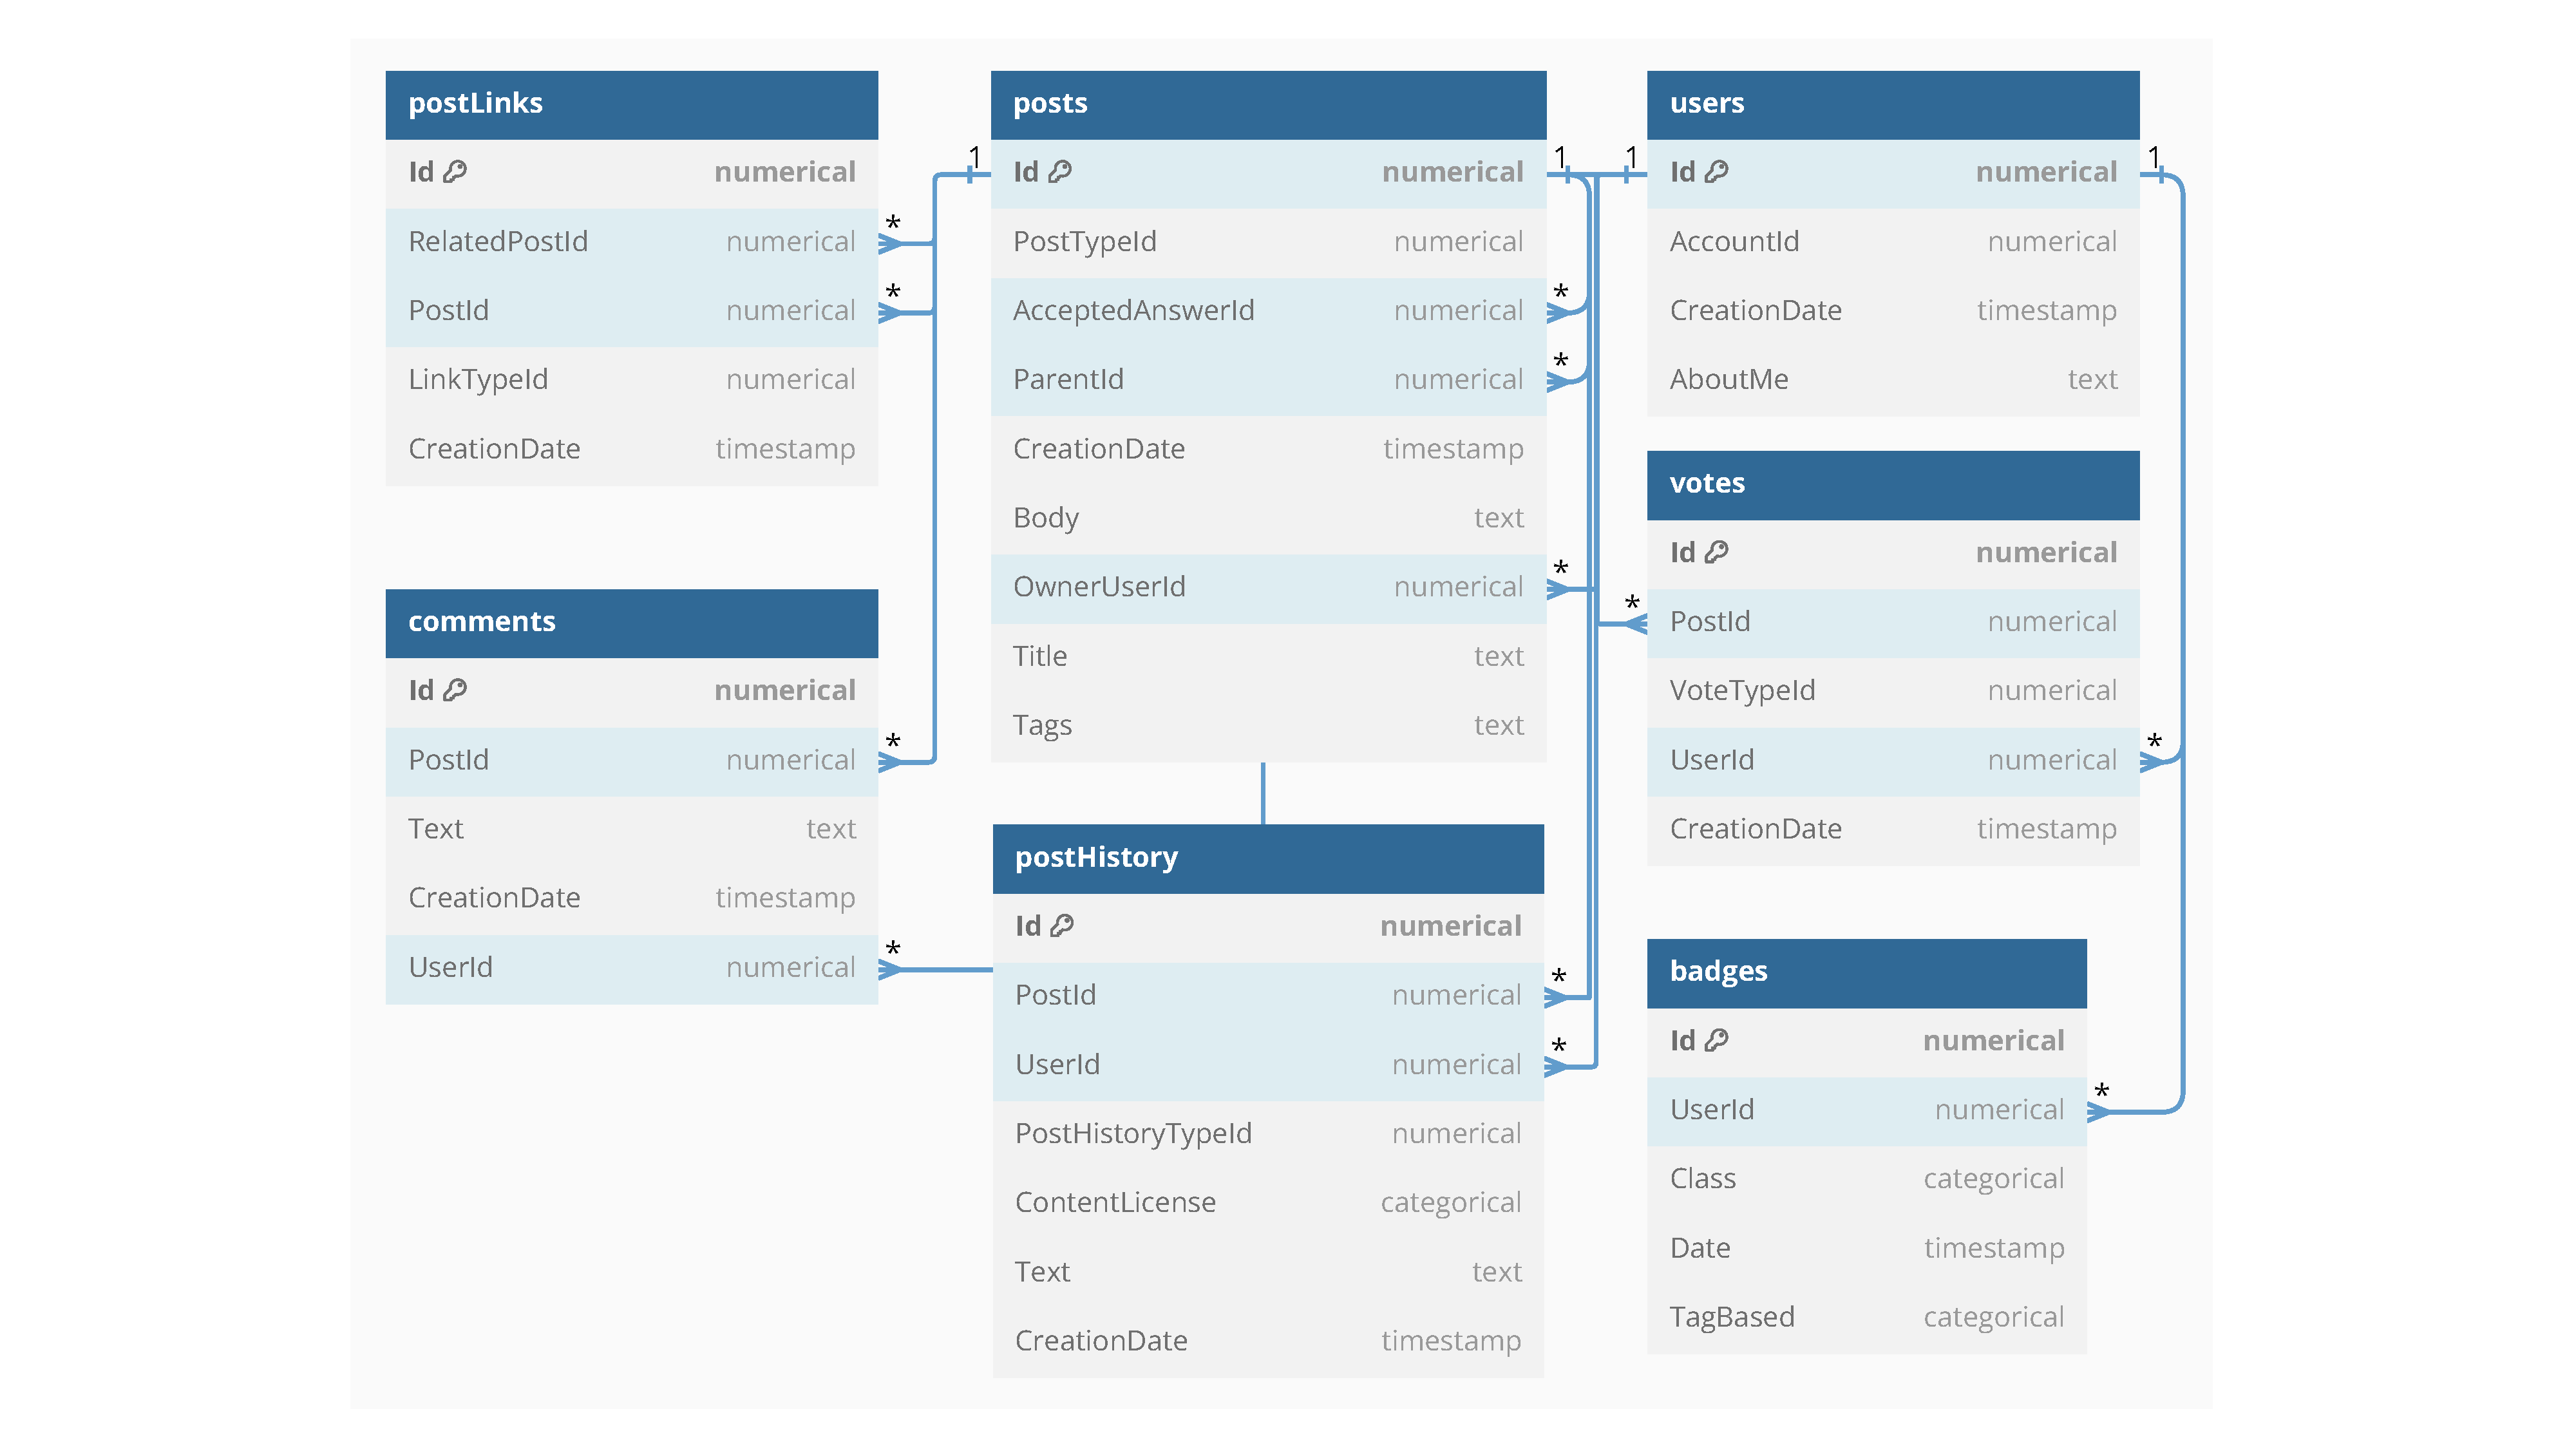
\includegraphics[width=0.9\textwidth]{figs/rel-stack.pdf}
    \caption{\stackex database diagram.}
    \label{fig:stack-db}
\end{figure}

\begin{figure}[H]
    \centering
    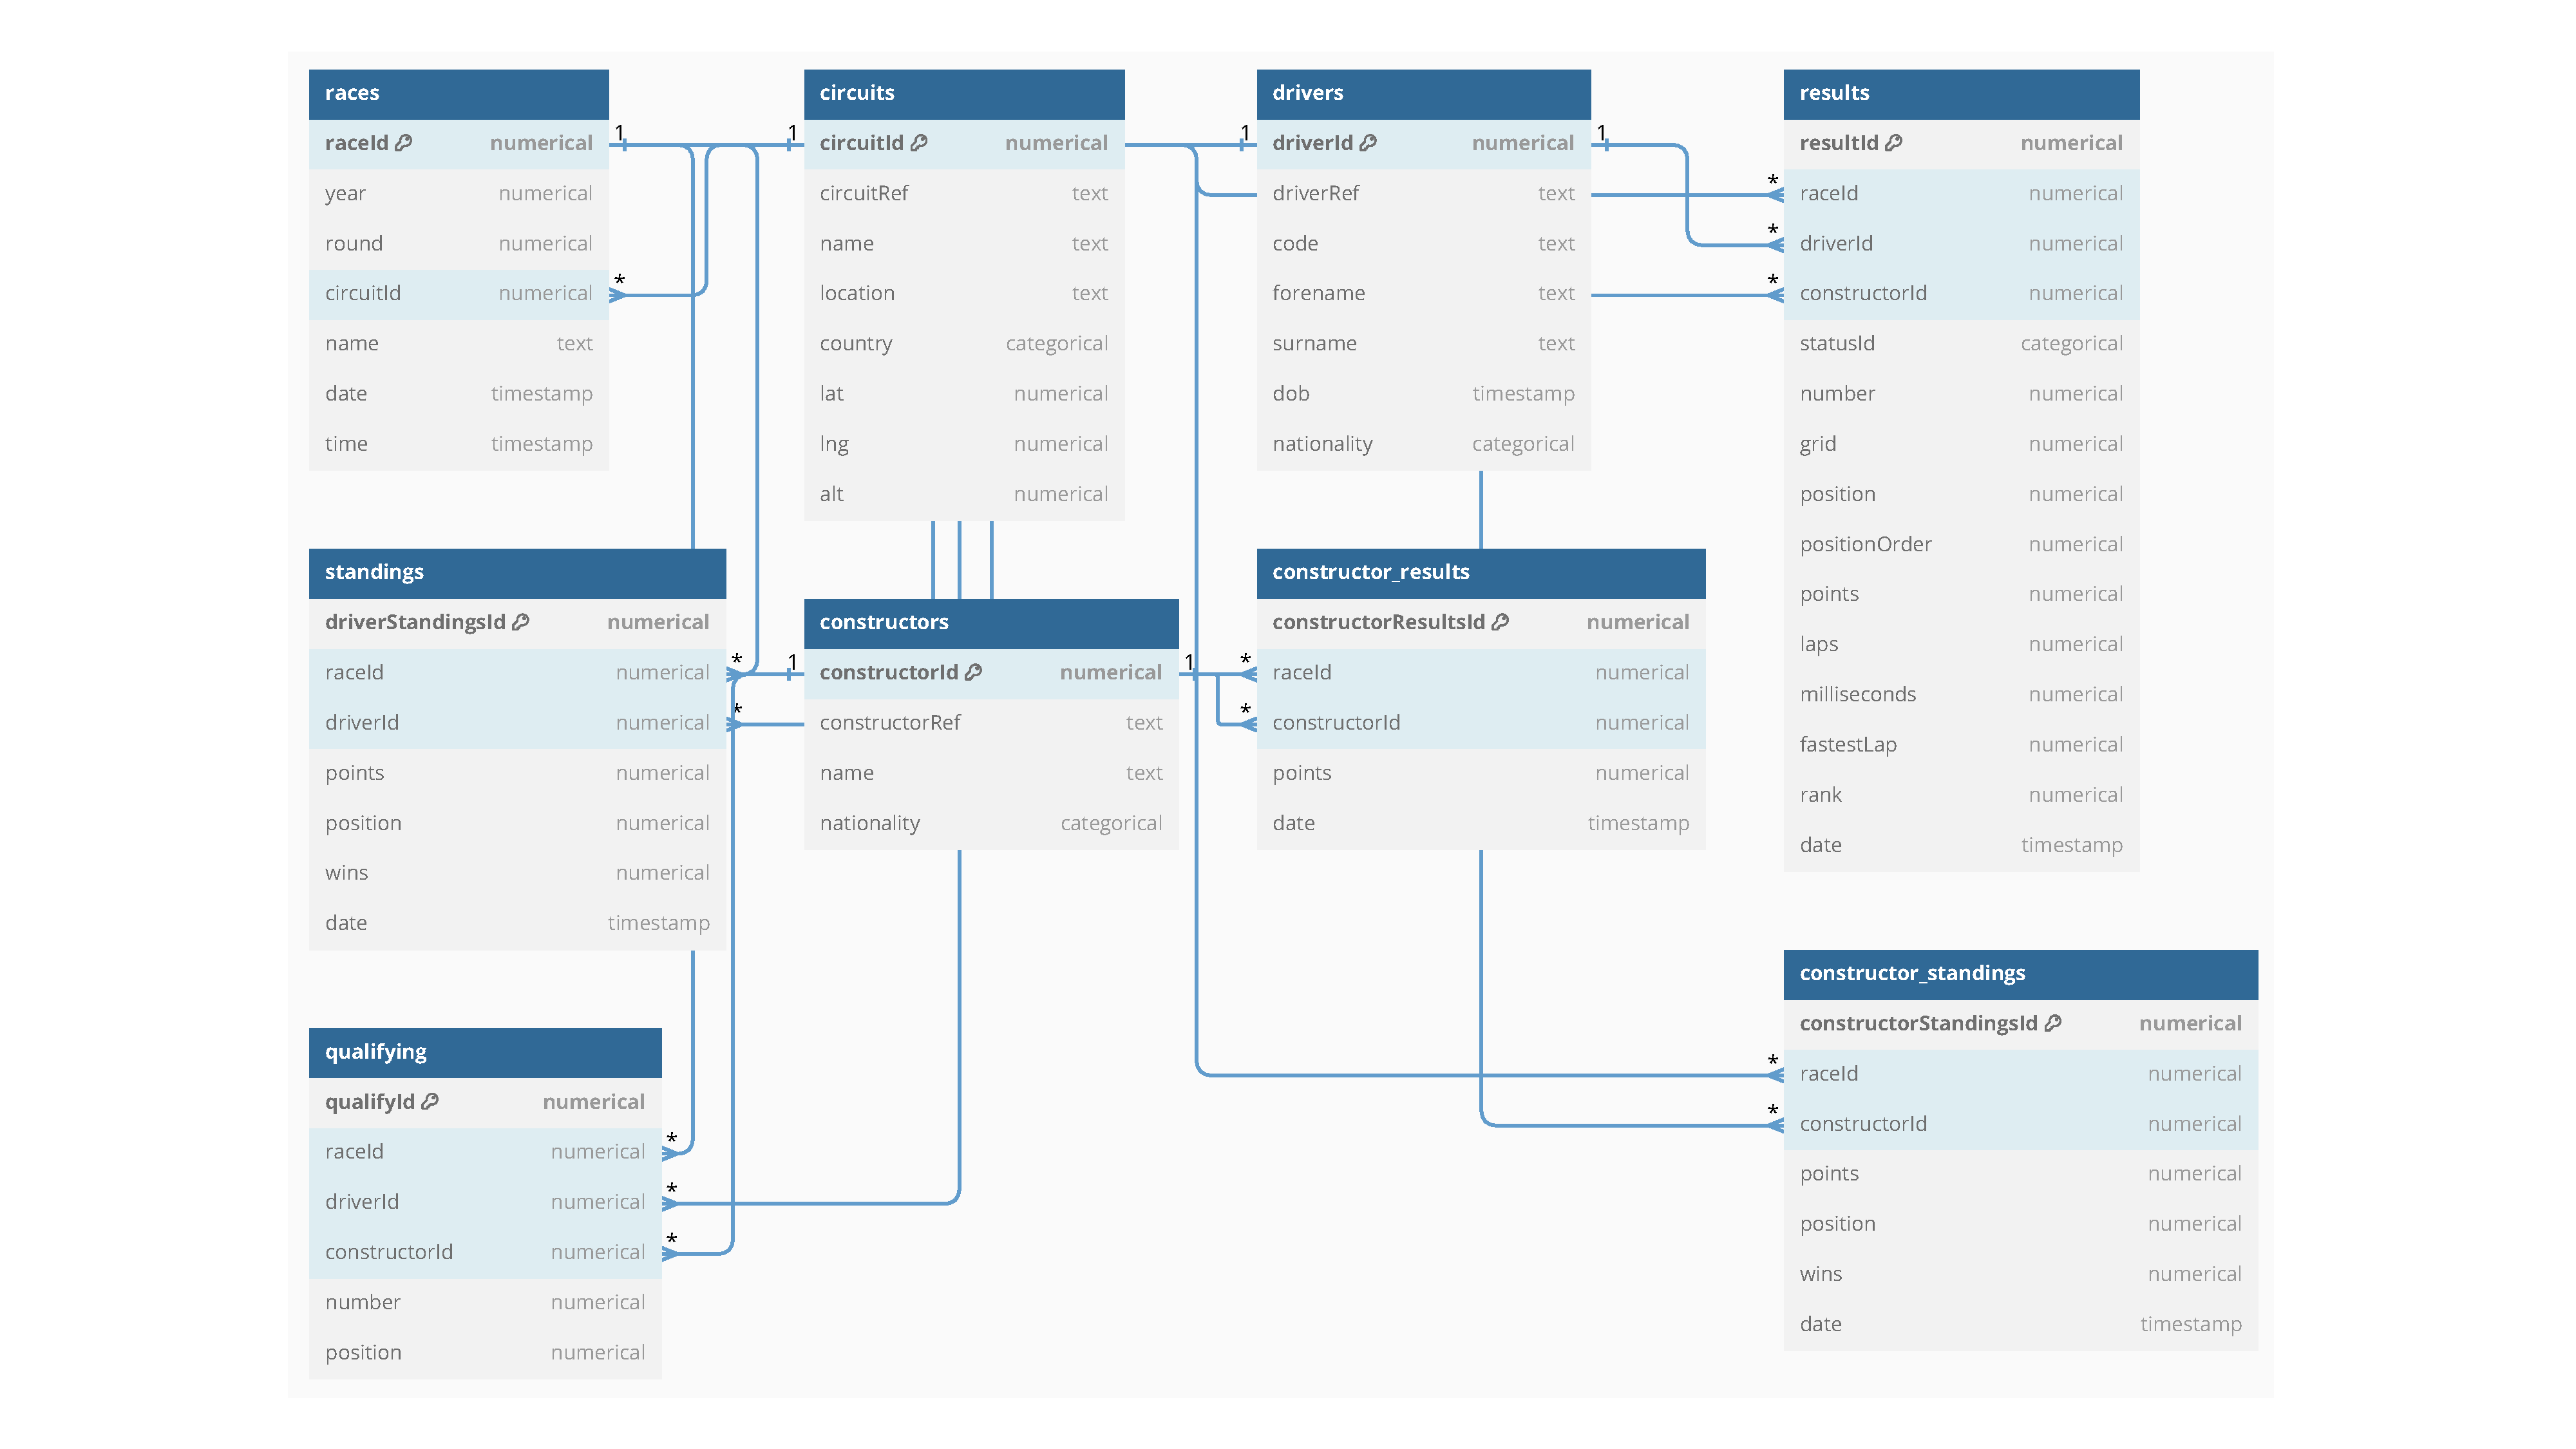
\includegraphics[width=0.9\textwidth]{figs/rel-f1.pdf}
    \caption{\fone database diagram.}
    \label{fig:f1-db}
\end{figure}


\begin{figure}[H]
    \centering
    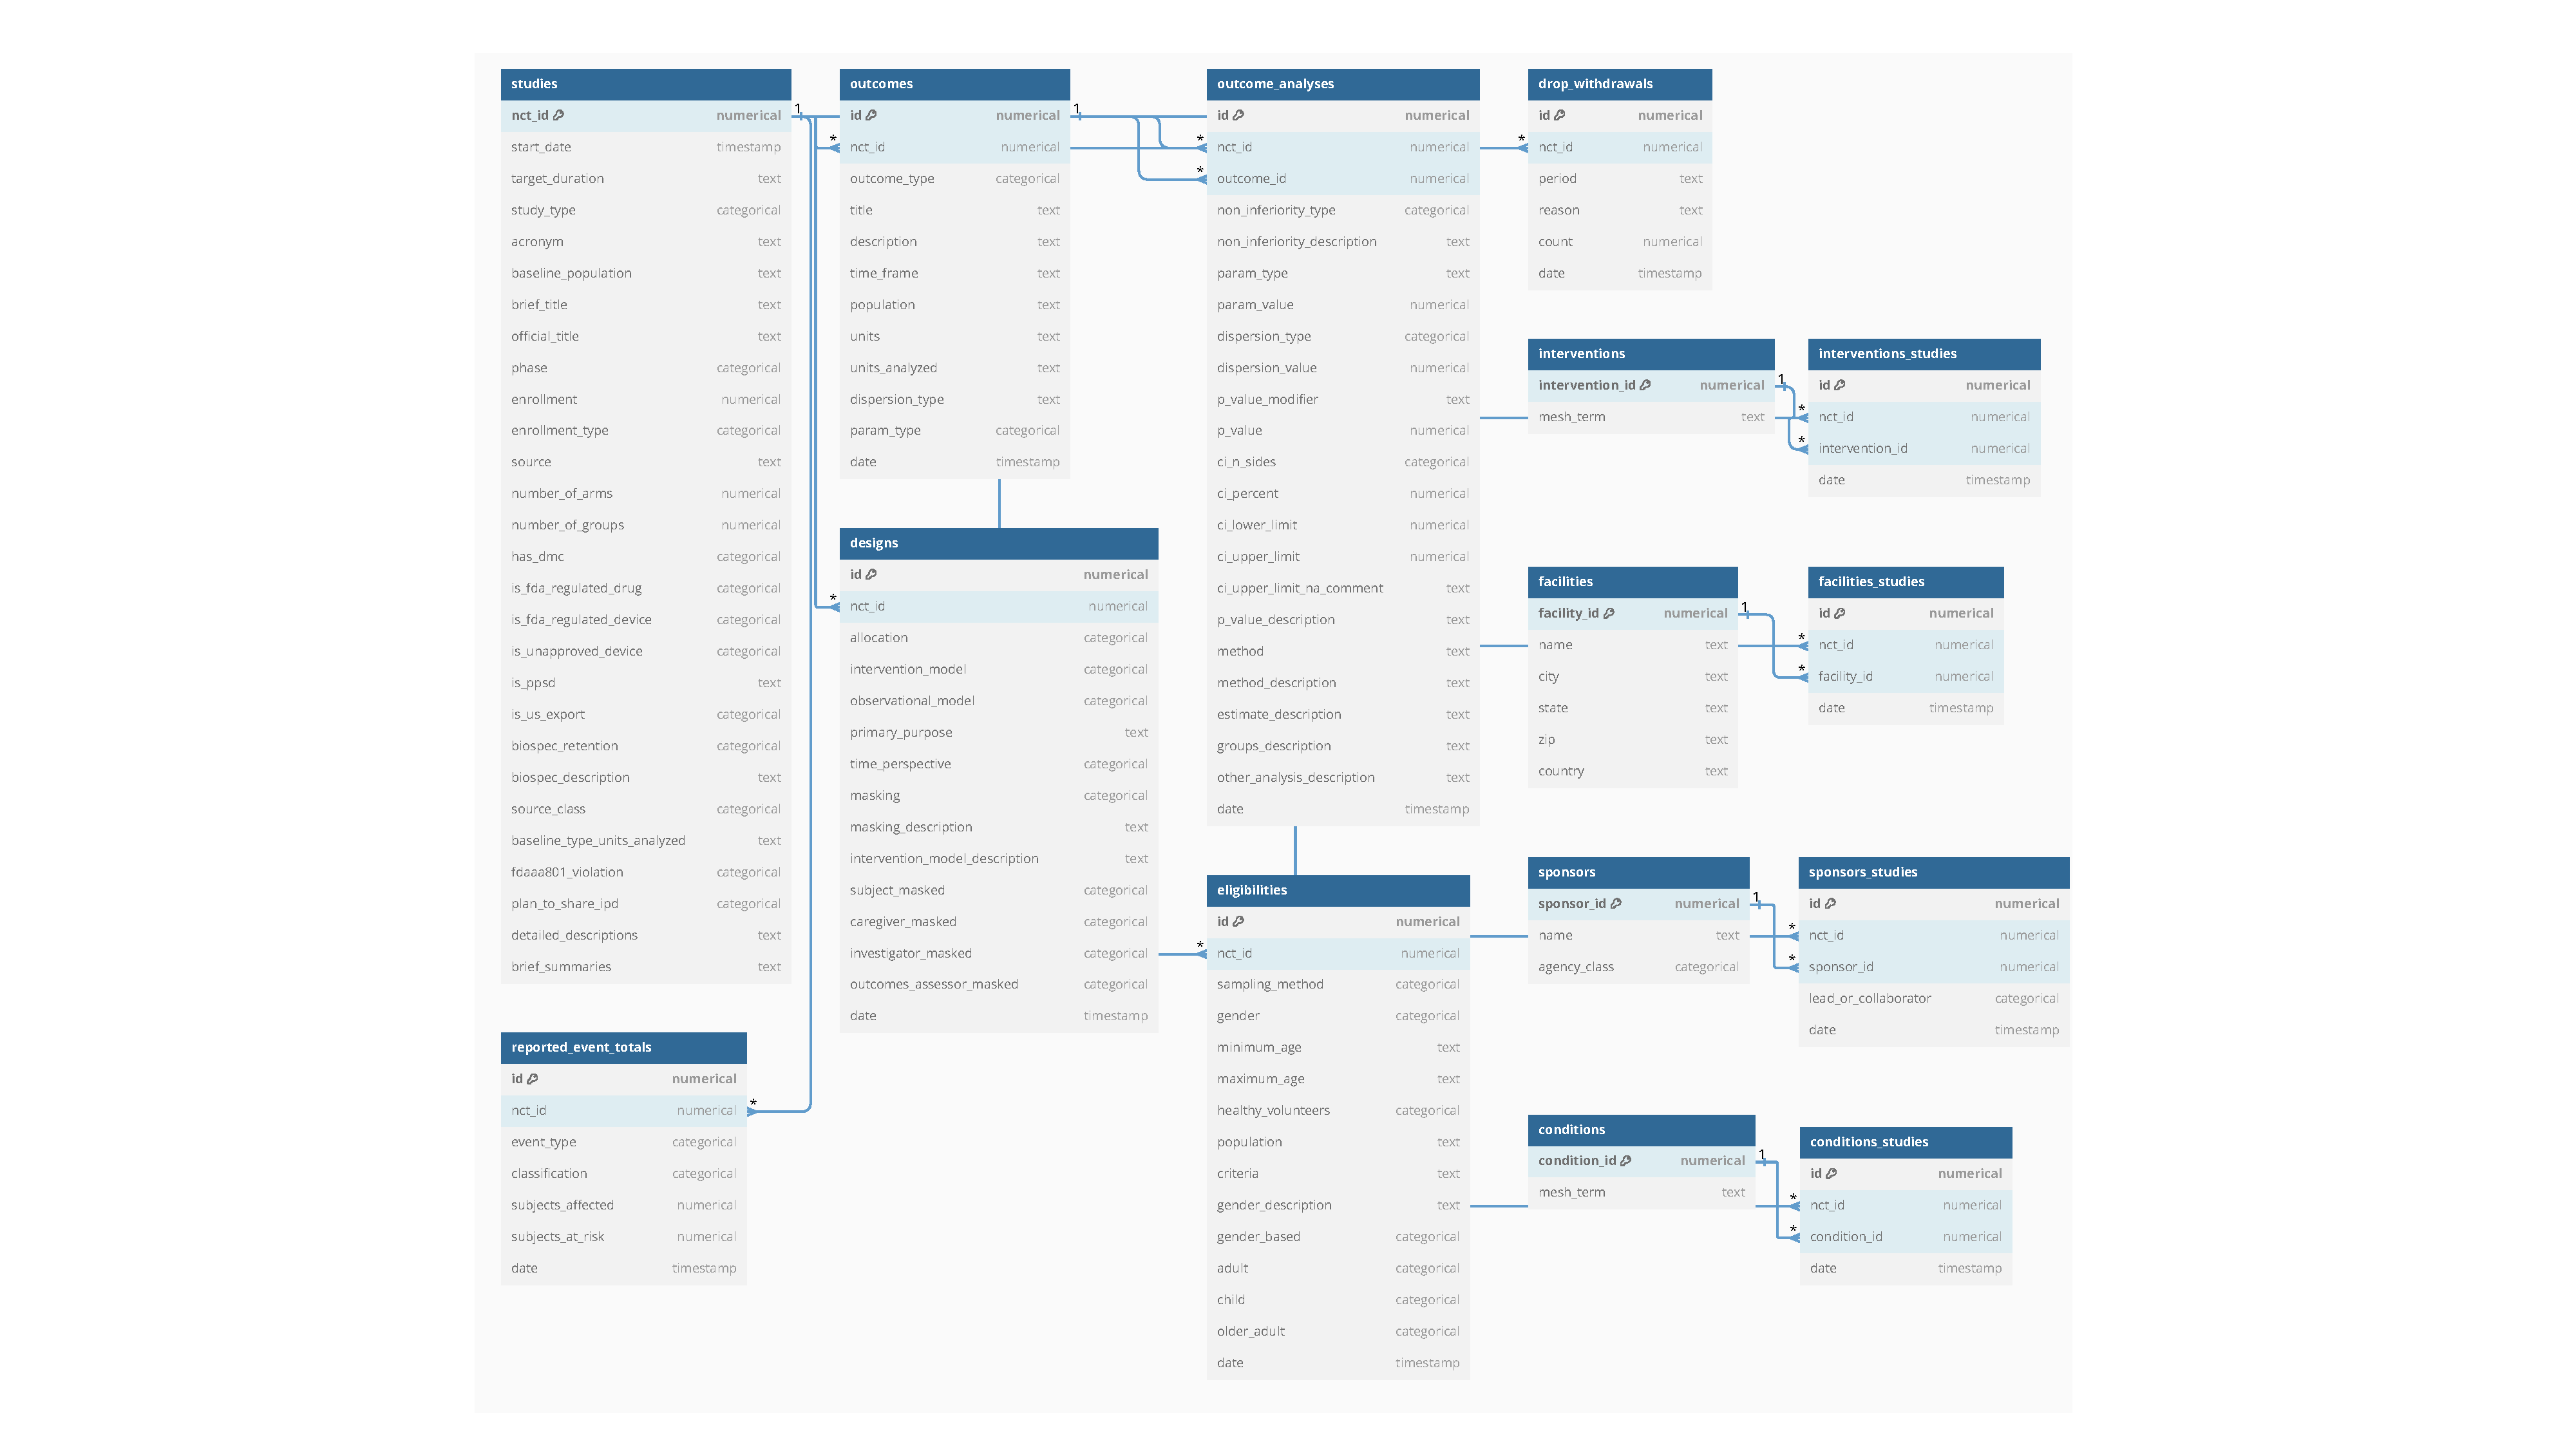
\includegraphics[width=1\textwidth]{figs/rel-trial.pdf}
    \caption{\trials database diagram.}
    \label{fig:trial-db}
\end{figure}


\begin{figure}[H]
    \centering
    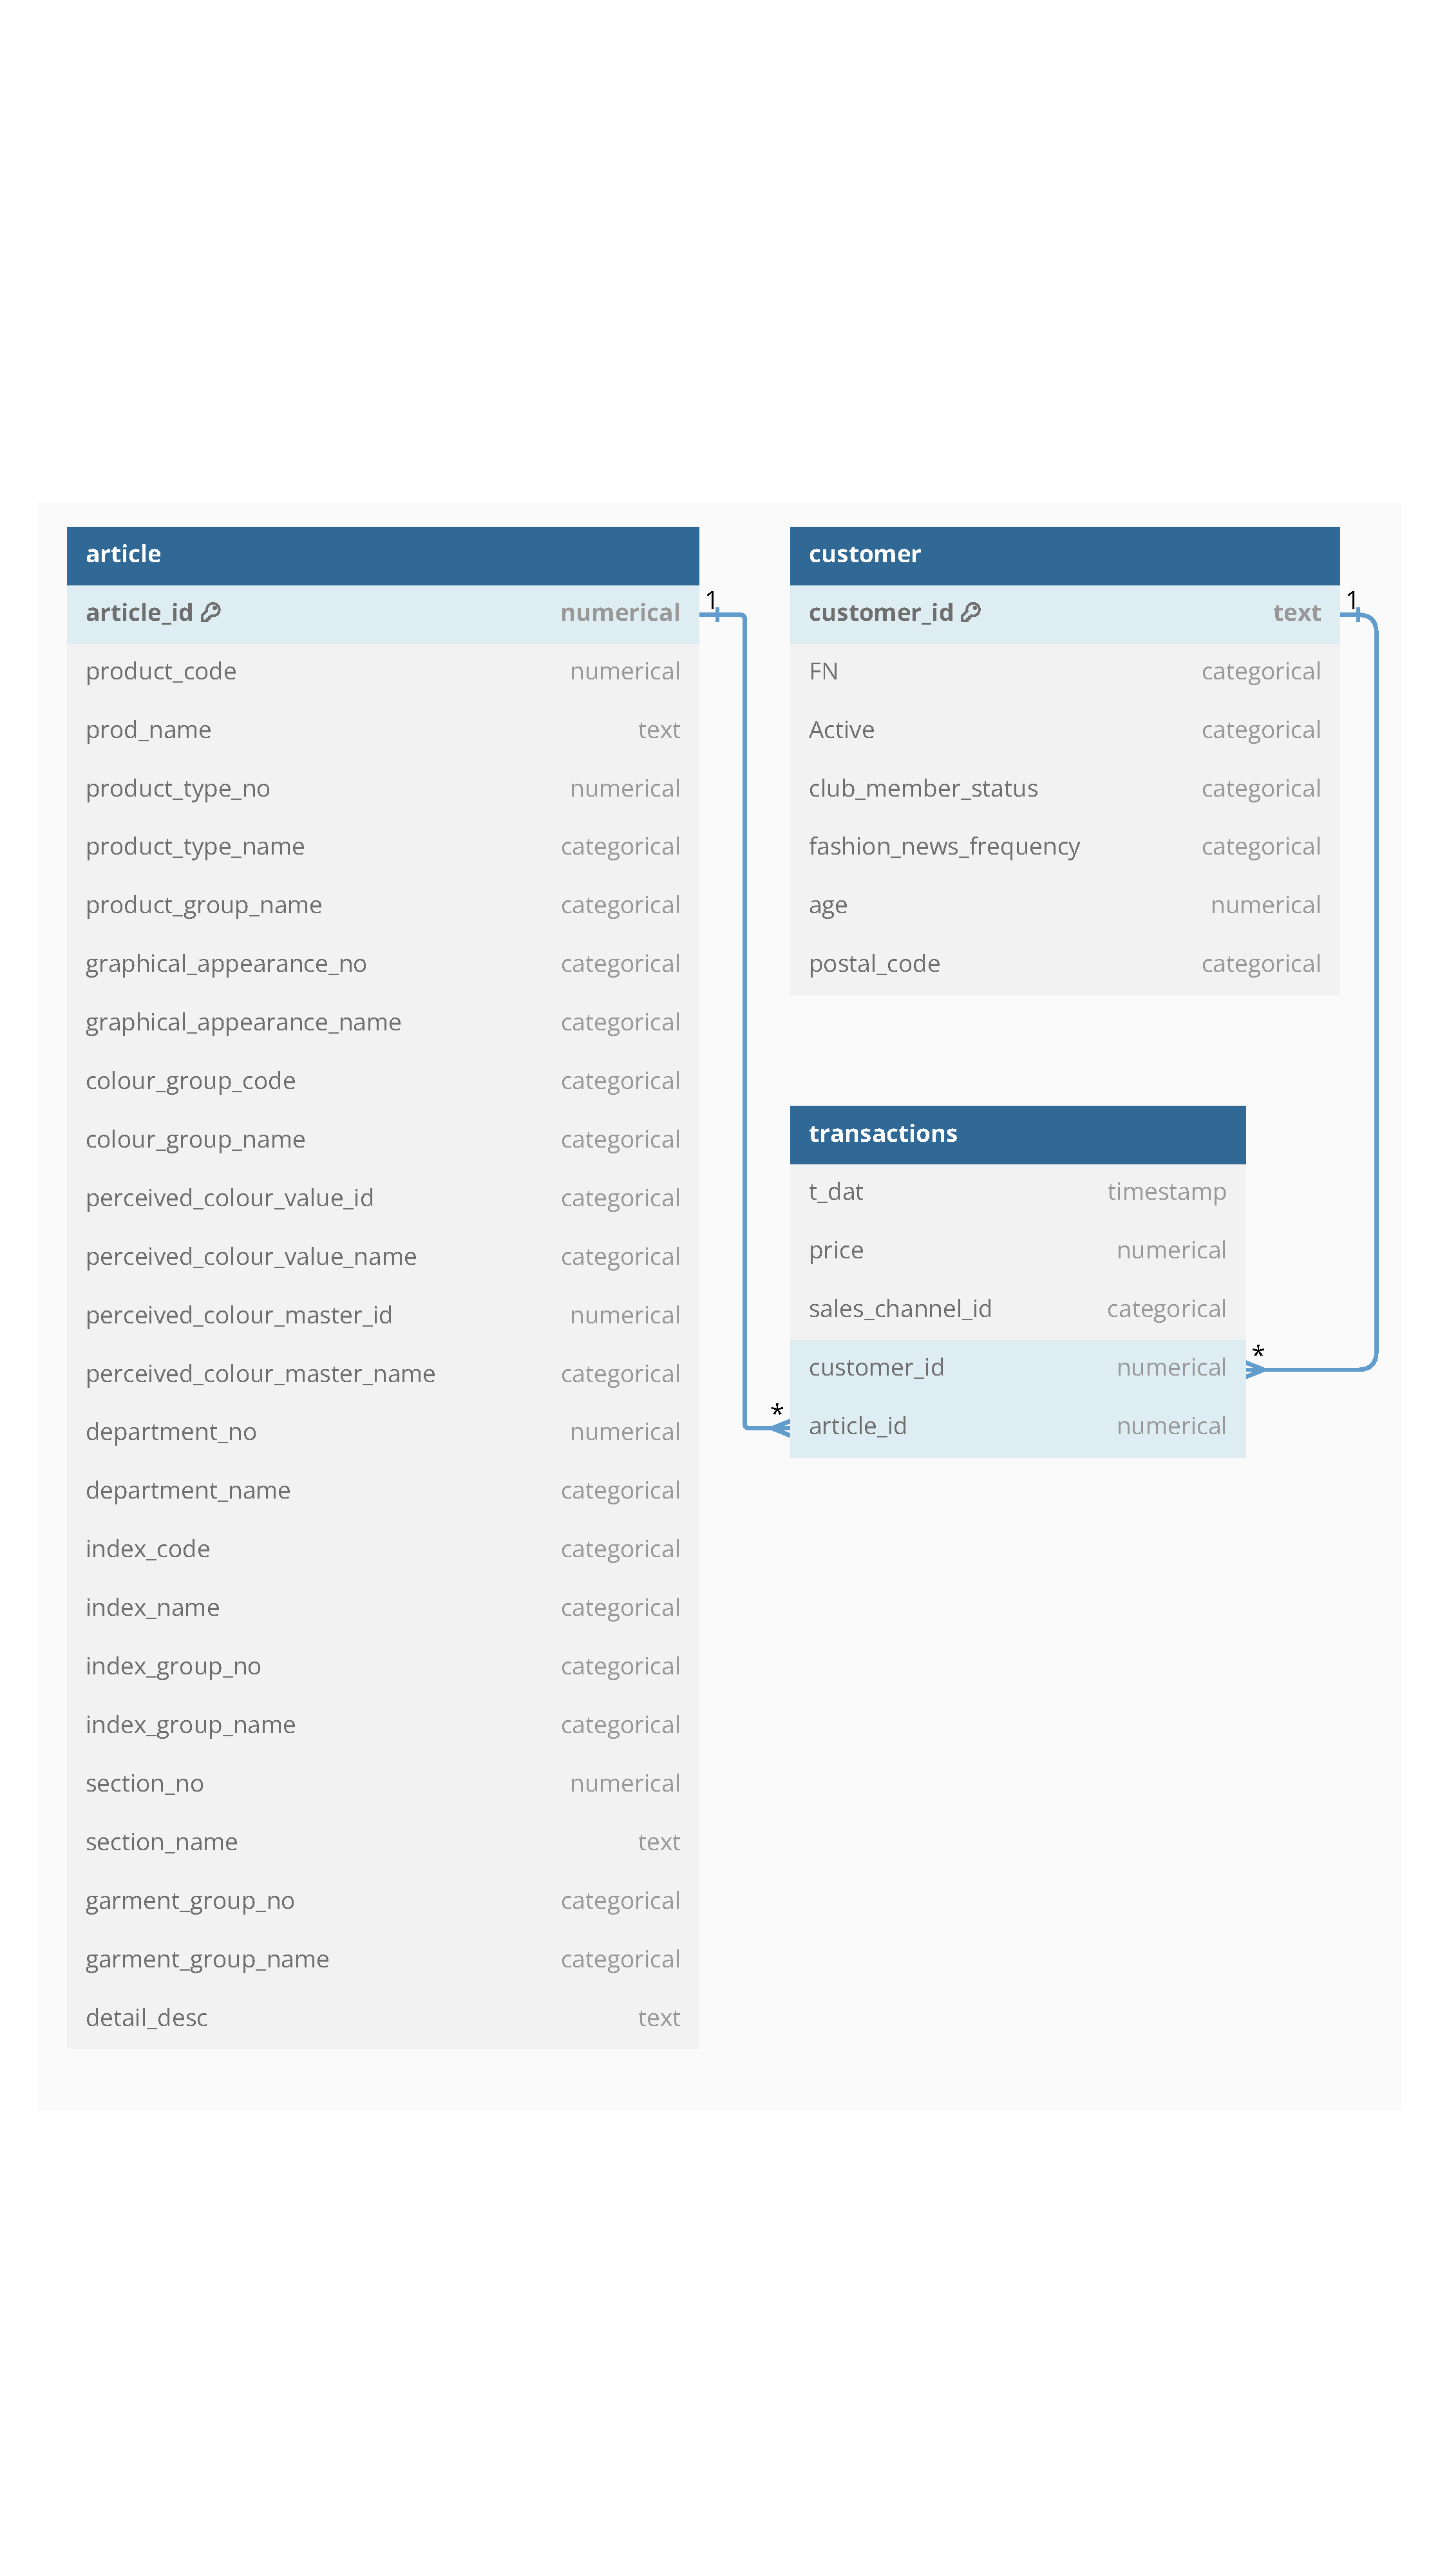
\includegraphics[width=0.8\textwidth]{figs/rel-hm.pdf}
    \caption{\handm database diagram.}
    \label{fig:hm-db}
\end{figure}

\begin{figure}[H]
    \centering
    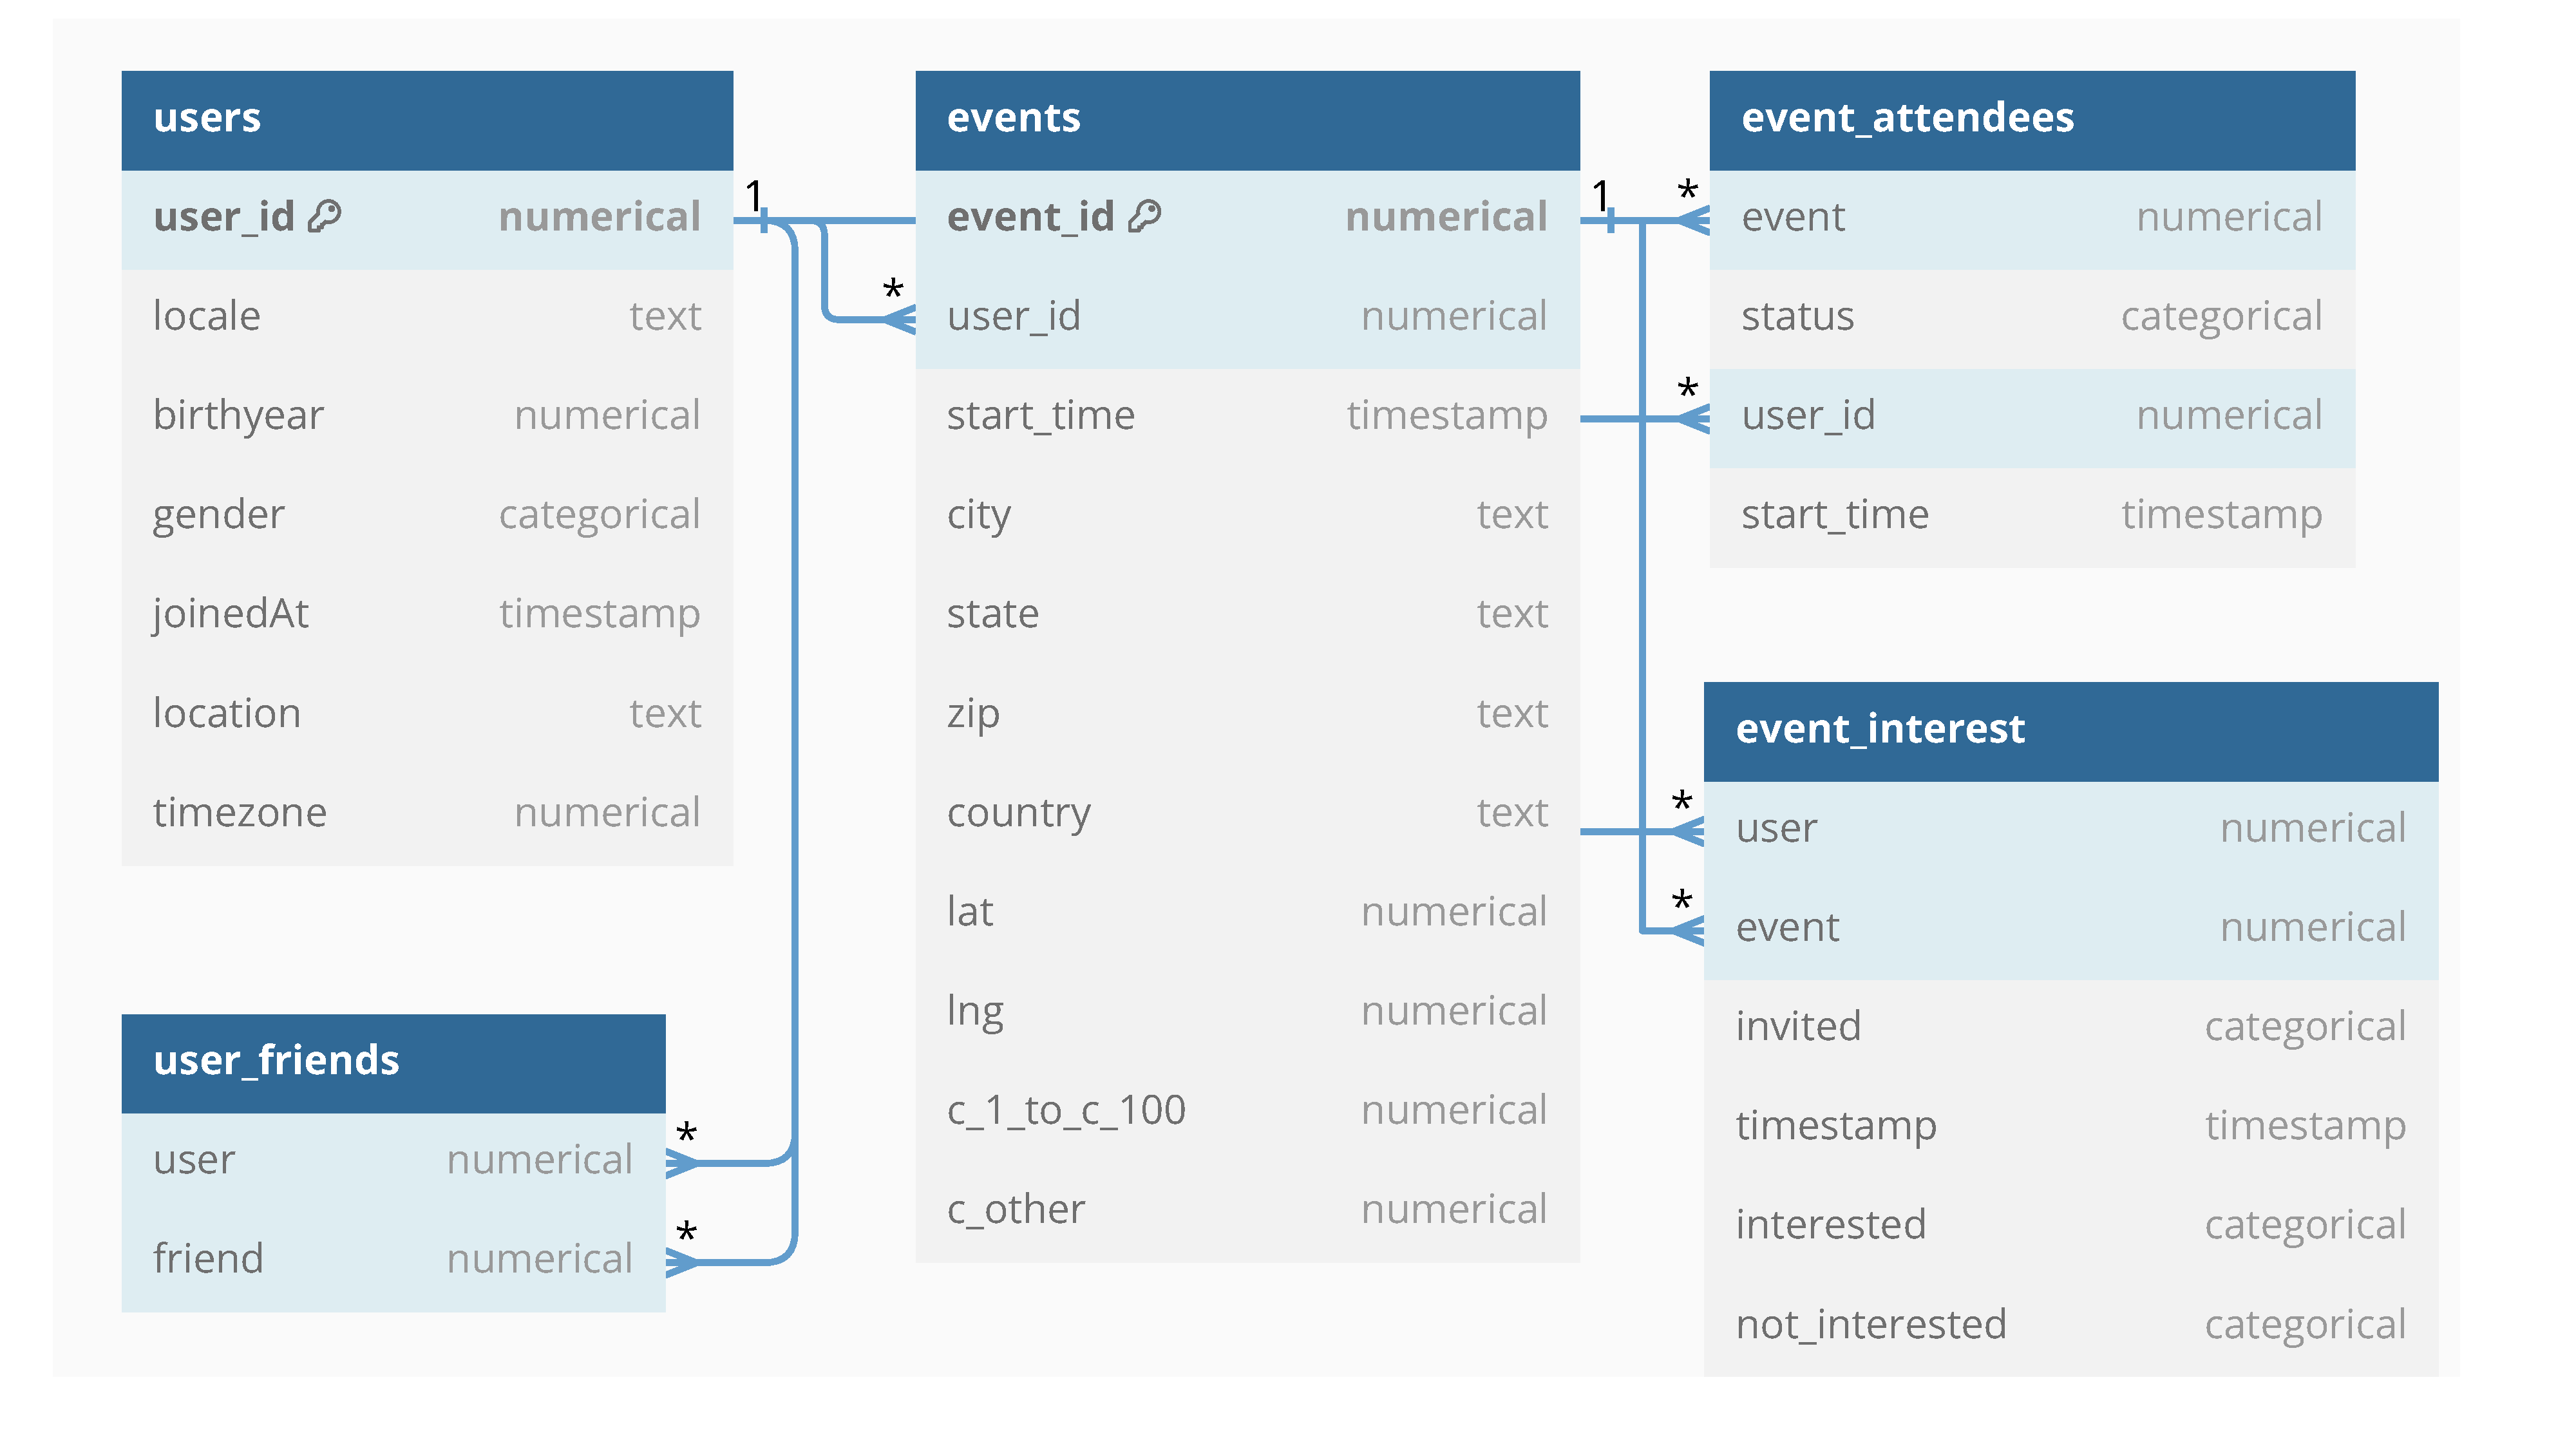
\includegraphics[width=1\textwidth]{figs/rel-event.pdf}
    \caption{\event database diagram.}
    \label{fig:event-db}
\end{figure}


\begin{figure}[H]
    \centering
    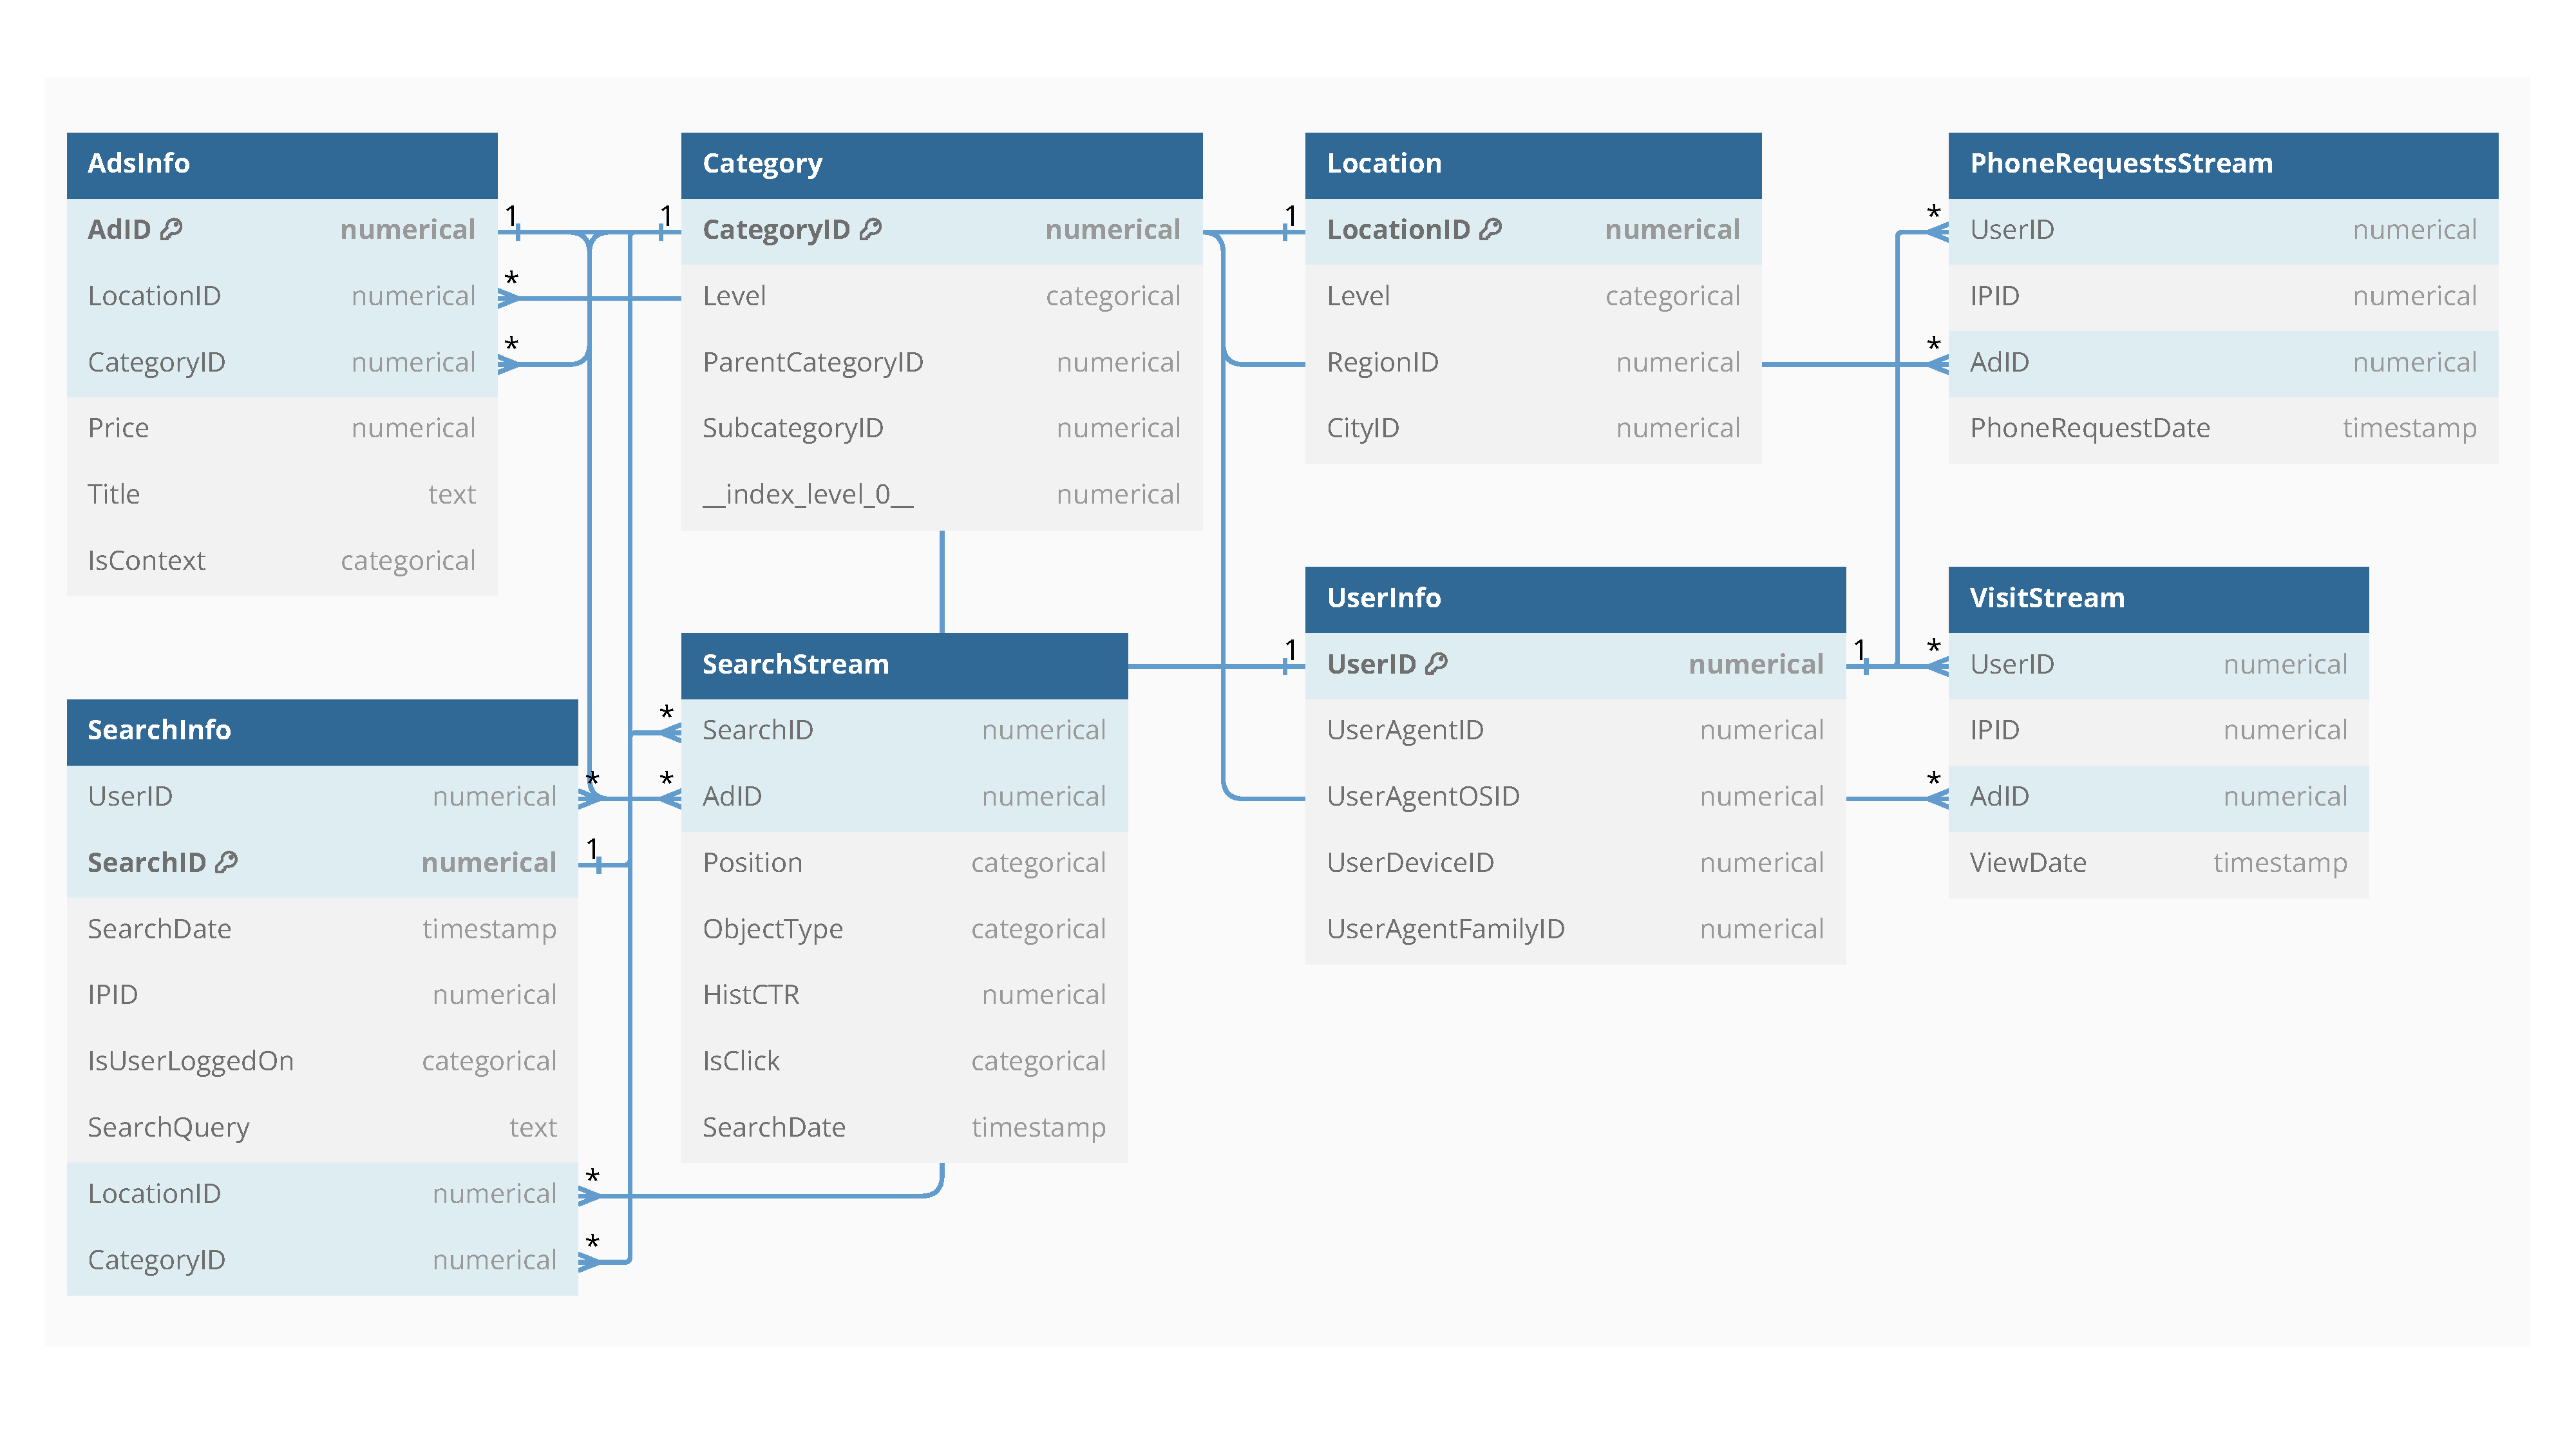
\includegraphics[width=1\textwidth]{figs/rel-avito.pdf}
    \caption{\avito database diagram.}
    \label{fig:avito-db}
\end{figure}